% CSCI 580 Project - Fall 2015 - Western Washington University
% Author: Sam Pollard (pollars at students dot wwu dot edu)
% Last Modified: December 4, 2015
% Code taken from Geof Matthews (github.com/geofmatthews/csci480)

\documentclass[12pt]{article}
\usepackage[top=1.25in, bottom=1.25in, right=1in, left=0.5in, headheight=15pt]{geometry}

\usepackage{amsmath, amssymb, amsthm}
\usepackage{fancyhdr}
\usepackage{fancyvrb}
\usepackage{url}

\usepackage{graphicx}
\DeclareGraphicsExtensions{.png}

\usepackage{tikz}
\usepackage{tkz-euclide}
\usetikzlibrary{decorations.pathreplacing}
\usetkzobj{all}
\usepackage{pgfplots}
\pgfplotsset{compat=1.11}

\renewcommand{\headrulewidth}{0pt}
\setlength{\headheight}{30pt}

\pagestyle{fancy}
\lhead{Sam Pollard}
\rhead{CS 580 -- Fall 2015 -- Matthews}
\cfoot{\thepage}

% To indent new paragraphs in an enumerated list. (my enum items are rather long!)
\usepackage{enumitem}
\setlist{parsep=0pt}
\setenumerate{listparindent=\parindent}

% My personal macros for commonly used commands
\newcommand{\real}{\mathbb{R}}
\newcommand{\setdiff}{\backslash}
\renewcommand{\natural}{\mathbb{N}} % Not the musical natural
\newcommand{\claim}{\vspace{10pt}\emph{Claim. }}
\newcommand{\mand}{\textnormal{ and }}
\newcommand{\mor}{\textnormal{ or }}
\newcommand{\D}{\textnormal{d}}
\newcommand{\cU}{\mathcal{U}}
\newcommand{\cO}{\mathcal{O}}
\DeclareMathOperator{\ext}{ext}
\DeclareMathOperator{\id}{id}
\newcommand*\diff{\mathop{}\!\mathrm{d}}

\title{Procedurally Generated Script}
\author{Sam Pollard \\ Western Washington University}
\date{CS 580 -- Fall 2015 -- Geoff Matthews \\ \today}

\begin{document}
\maketitle

\begin{figure}[ht]
	\vspace{-30pt}
	\centering
	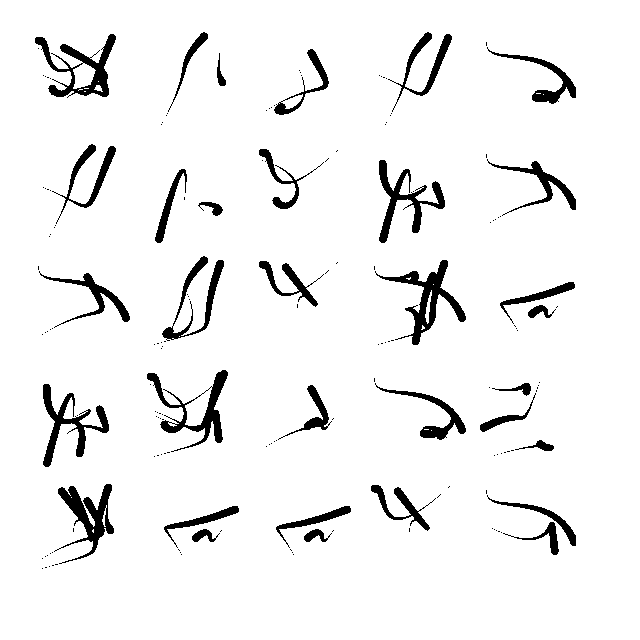
\includegraphics[width=3.5in]{sample.png}
	\vspace{-18pt}
	\caption{Random characters using $T(t) = 0.1(1-t)$.}
	\label{sample}
\end{figure}

\section{Introduction}
We wish to model an arbitrary handwriting system that may be used to procedurally generate realistic looking handwriting. Once the parameters are specified this model aims to output pseudorandom sequences of characters which look realistic without any further intervention.

This model is in line with the Metafont language, which models characters as curves with finite width. This is in contrast to languages like PostScript and TrueType which describe the outline of each character.

This decision is based on the assumption the hand draws curves with thickness $\epsilon$ which may change based on physical attributes of the curve. There may be many factors which affect the thickness of a curve so in general we define a function $T : [0,1] \to [0,\infty)$. We denote $\epsilon$ the output of this function. The $T$ used for in Fig.~\ref{bezier} is a constant function.

\begin{figure}
\centering
\begin{tikzpicture}[scale=2]%,cap=round,>=latex]
	\coordinate (p0) at (0,0);
	\coordinate (p1) at (-1,2);
	\coordinate (p2) at (1,2);
	\coordinate (p3) at (1,1);
	\coordinate (qhat) at (-0.29,1);
	\coordinate (uv) at (-1,1.07);
	\coordinate (tangent) at (-0.24,1.5);
    % Draw a border around the curve
    \draw[double distance=14mm,line width=1pt,line join=round,line cap=round,blue] (p0) .. controls (p1) and (p2) .. (p3);
	% Draw the bezier curve
	\draw[line width=1pt] (p0) .. controls (p1) and (p2) .. (p3);
	% Mark and label the control points
    \filldraw[red] (p0) circle[radius=1.5pt] node[black, anchor=west, yshift=-2.5mm] {$p_0$};
    \filldraw[red] (p1) circle[radius=1.5pt] node[black, anchor=west, yshift=-2.5mm] {$p_1$};
    \filldraw[red] (p2) circle[radius=1.5pt] node[black, anchor=west, yshift=-2.5mm] {$p_2$};
    \filldraw[red] (p3) circle[radius=1.5pt] node[black, anchor=west, yshift=-2.5mm] {$p_3$};
    % Label the point and its projection
    \filldraw[green] (qhat) circle[radius=1.5pt] node[black, anchor=west, yshift=-0.5mm] {$\hat{q}$};
    \tkzMarkRightAngle[size=0.15](uv,qhat,tangent);
    \filldraw[black] (uv) circle[radius=1.5pt] node[anchor=east] {$q$} -- (qhat);
\end{tikzpicture}
\caption{A sample bezier curve with a constant thickness $\epsilon$.}
\label{bezier}
\end{figure}

To model each stroke (or part of a stroke), we define a B\'ezier curve $B(t)$ for $t \in [0,1]$ by four control points $p_0$, $p_1$, $p_2$, $p_3 \in \mathbb{R}^2$. For our purposes, the control points are in $[0,1]^2$. To clarify notation, $B(t) = \begin{bmatrix} B_u(t) & B_v(t) \end{bmatrix}^T$

To determine whether this point lies inside or outside the region, we must first express $B(t)$ implicitly. We define

\[
	B(t) = (1 - t)^3 p_0 + 3(1 - t)^2 t p_1 + 3(1 - t)t^2 p_2 + t^3 p_3
\]
where $p_i = (u_i, v_i)$, the coordinates of each control point.

Next, we determine if a given point $q = (u,v)$ lies inside of the stroke. That is, there exists some $\hat{q} = B(\hat{t})$ such that $||q - \hat{q}||_2 < T(\hat{t})$. One way to accomplish this is to find the nearest point to $q$ on $B$, denoted $\hat{q} = (\hat{u}, \hat{v})$. Since $B$ is a parametrized curve there exists a $\hat{t}$ such that $B(\hat{t}) = \hat{q}$. Then, $q$ is contained in the stroke if and only if $||q - \hat{q}||_2 < \epsilon$ for some $\hat{t} \in [0,1]$. We find one such $\hat{q}$ by observing the vector $\hat{q} - q$ is orthogonal to $\diff B / \diff t$. There may be multiple such $\hat{q}$. In this case, we simply choose the $\hat{q}$ with the smallest distance to $q$. There may also exist multiple $\hat{t} \in [0,1]$ such that $B(\hat{t}) = \hat{q}$. Of these, we choose the $\hat{t}$ such that $||q - \hat{q}||_2$ is minimized. So we solve for $t$ in
\begin{align}
 0 &= \hat{q} \cdot \frac{\diff B}{\diff t} \nonumber \\
  &= B_u(t)\frac{\diff B_u}{\diff t}(t) + B_v(t)\frac{\diff B_v}{\diff t}(t) \label{poly}
\end{align}
which amounts to finding the real roots of a fifth-order polynomial. We know fifth order polynomials have at least one real root and at most five real roots. Therefore, the problem of nonunique $\hat{t}$ and $\hat{q}$ will require at most finding these five roots and computing the minimimum distance for each $\hat{t}$. For the exact formula of this polynomial see the attached Python code.

\section{The \texttt{Handwriting} Texture}
We define a texture as a function which takes as input a $(u,v)$ coordinate and returns either another texture (which can in turn be evaluated at $(u,v)$) or an RGB color value. In the case of handwriting, we return one texture if $(u,v)$ is inside the curve and a second texture otherwise. The $T$ function described in Section 1 is known as the brush in the \texttt{Handwriting} class. This implementation defines $T$ as a function only of the B\'ezier curve's parameter $t$.

A given \texttt{Handwriting} instance has a list of characters defined by zero or more B\'ezier curves. Each character has all of its B\'ezier curves (also called strokes) contained in $[0,1]^2$. Specifically, for any curve, all of its control points are in $[0,1]^2$. For each $(u,v)$ texture coordinate, we determine if $\hat{q}$ is contained in any of the strokes in the nearby characters.

\begin{figure}[ht]
\centering
\begin{tikzpicture}[scale=2, fill opacity=0.4, draw opacity=1]
	\filldraw[fill=yellow!60!white, draw=black] (-0.75,0) rectangle (0.25,1);
	\filldraw[fill=orange!60!white, draw=black] (-0.75,0.75) rectangle (0.25,1.75);
	\filldraw[fill=green!60!white, draw=black] (0,0.75) rectangle (1,1.75);
	\filldraw[fill=blue!60!white, draw=black] (0,0) rectangle (1,1);
	% The gray areas on the bottom right sides
	\filldraw[fill=black!60!white, draw=black, dashed] (0.75,1.75) rectangle (1,0);
	\filldraw[fill=black!60!white, draw=black, dashed] (-0.75,0) rectangle (1,0.25);
	\draw[red, very thick] (0,1) rectangle (0.75,0.25);
	% Label
	\draw [decorate,decoration={brace},yshift=1pt] (0,1.75) -- (0.25,1.75) node [black, midway, yshift=8pt, opacity=1] {$h$};
	\draw [decorate,decoration={brace},xshift=1pt] (1,1) -- (1,0.75) node [black, midway, opacity=1, xshift=6pt] {$s$};
	\draw (0.5, 0.5) [black, opacity=1] node {$C_c$};
	\draw (-0.25, 0.5) [opacity=1] node {$C_l$};
	\draw (-0.25, 1.25) [opacity=1] node {$C_{al}$};
	\draw (0.5, 1.25) [opacity=1] node {$C_a$};
\end{tikzpicture}
\caption{A point inside of the red box may be inside any of $C_{al}$, $C_c$, $C_a$, or $C_l$.}
\label{charboxes}
\end{figure}

To make the writing look more natural, we wish to have characters overlap. This may be specified with $h$ and $s$. If $h,s \in [0,0.5)$ then there will never be more than four characters present in any given point. Consider Fig.~\ref{charboxes}. Given that each colored box is $[0,1]^2$ and we stack each character so that the overlap horizontally is $h$ and the overlap vertically is $s$, for each character $C$ we must also check the characters to the left, above, and diagonally above and to the left of $C$. We do not need to check the other surrounding characters because these will be checked if $(u,v)$ is in the first $[1-h] \times [1-s]$ box of the next character. For the center character $C_c$ this box is outlined with thick, red lines in Fig.~\ref{charboxes}.

Then, given some coordinate $(u,v)$ we transform the coordinate so we can determine which character box the point is contained in as well as where inside the box. This is achieved with the functions
\begin{align}
	g_u(u) &= u + h \left\lfloor \frac{u}{1-h} \right\rfloor \label{gu} \\
	g_v(v) &= u + s \left\lfloor \frac{v}{1-s} \right\rfloor. \label{gv} \\
	f_u(u) &= u + h \left\lfloor \frac{u - h}{1-h} \right\rfloor \label{fu} \\
	f_v(v) &= v + s \left\lfloor \frac{v - s}{1-s} \right\rfloor \label{fv}
\end{align}
Equations \eqref{gu} and \eqref{gv} transform from a $(u,v)$ coordinate to the position in the overlapped characters, where the ingetral parts of $(g_u(u), g_v(v))$ determine the character and the decimal parts determine the coordinate in that character. However, this overlapping lattice may have multiple characters for a given point. Thus for each point $u,v$ we must check $(g_u(u), g_v(v))$, $(g_u(u), f_v(v))$, $(f_u(u), g_v(v))$, and $(f_u(u), f_v(v))$. These determine the coordinates inside of $C_c$, $C_a$, $C_l$, and $C_{al}$ from Fig.~\ref{charboxes}, respectively. The plots of \eqref{gu} and \eqref{fu} are shown in Fig.~\ref{transformplot}. Notice this is only along one axis and there is overlap of these functions on the domain $n + [h, 1-h]$ for $n \in \{0, 1, 2, \dots \}$.

\begin{figure}[ht]
\centering
\begin{tikzpicture}
	\begin{axis}[
			xlabel=$u$,
			ylabel=Overlayed $u$,
			legend cell align=left, legend pos=north west,
			legend entries={$g_u(u)$, $f_u(u)$}
		]
		\addplot[line width=2pt, blue, opacity=0.5, domain=0:0.74999, samples=2] {x + (0.25)*floor(x/0.75)};
		\addplot[line width=2pt, red, opacity=0.5, domain=0.25:1, samples=20] {x + (0.25)*floor((x-0.25)/0.75)};
		\addplot[line width=2pt, blue, opacity=0.5, domain=0.75:1.4999, samples=2] {x + (0.25)*floor(x/0.75)};
		\addplot[line width=2pt, red, opacity=0.5, domain=1.0:1.749, samples=20] {x + (0.25)*floor((x-0.25)/0.75)};
		\addplot[line width=2pt, blue, opacity=0.5, domain=1.5:1.75, samples=2] {x + (0.25)*floor(x/0.75)};
	\end{axis}
\end{tikzpicture}
\caption{Plots of equations \eqref{gu} and \eqref{fu} with $h = 0.25$.}
\label{transformplot}
\end{figure}

\section{Lessons Learned}
This approach is rather complicated and limited. Using Equations \eqref{gu}--\eqref{fv}, characters must all have the same spacing between them. Furthermore, performing other improvements is difficult because those equations are required anywhere to transform from the character space to the texture space.

The open-endedness of this project makes it exciting but also slows progress progress. It is difficult to know which design choices will lead to favorable results and which are nebulous or do not produce anything useful.

\section{Future Work}
The ideas outlined here are ordered by decreasing importance. Generalizing how characters are positioned on the surface is the most important because without it further improvements become increasingly difficult.

\subsection{Generalizing Character Positioning}\label{generalize}
A more general approach to positioning the characters would be to use traditional computer graphics methods (see~\cite{pbrt}) and with each character associate a $3 \times 3$ transformation matrix. In general, this makes determining which characters to check at every point more difficult but a reasonable assumption with handwriting is the characters are roughly evenly-spaced. Thus, one could split up the image into a rectangular grid and each time a transformation is set, keep track of which boxes that character fits inside. This would be a good starting point to make future changes easier. This method is known as a grid acceleration structure and described in Chapter 4 of~\cite{pbrt}.

Another generalization would be to join multiple B\'ezier curves. In characters such as ``z,'' there are sharp curves but the letter itself is still ultimately one stroke. This requires continuity but not smoothness of the first derivative. Some characters require first derivative continuity such as the character ``s.'' This should also be supported. Lastly, we would also like $T$ to be continuous across an entire stroke instead of just one B\'ezier curve. This models one ``stroke'' as multiple B\'ezier curves and represents one unbroken line drawn by some writing utensil.

\subsection{Adding Tunable Parameters}
Other methods exist for generating human-looking handwriting from a character sequence, such as the company Bond (\url{http://bond.co}) and generation of handwriting using Recurrent Neural Networks (\cite{Graves:2013:RNN}). There has been some work done procedurally generating handwriting (\url{http://bwiklund.github.io/roboglyphics/}). However, there is little apart from designing an entire typeface which can allow for a completely automated, arbitrarily precise script system. The ultimate goal is to provide artists with a tool with many tunable parameters to give a large space of possible handwriting styles. Whether these are to emulate an alien language or human language is undetermined.

To accomplish this, more parameters should be implemented. The first would be the ability to connect characters together. This could better emulate cursive writing. For example, one could specify the mean, variance, minimum, and maximum word lengths to get a probability density of word lengths, which could in turn determine which characters to connect.

A ``curviness'' paramter would be useful in determining the appearance of the langauge. A value of zero would be completely straight lines, while increasing this would tend the middle control points $p_1$ and $p_2$ away from the line between $p_0$ and $p_3$.

Each handwritten character looks different. To add realism, a parameter could be specified which indicates how much each character is perturbed from its original specification. We wish to perturb the character such that it looks different but is still recognizable. This could consist of a weighted combination of the original character's control points with random control points. Other perturbations could be slight rotations, translations, shearing, and scaling. These could all be specified using the translation matrices described in Section~\ref{generalize}.

\subsection{Writing Utensil Modeling}
For a fountain pen, the thickness of the stroke depends on the minimum and maximum widths of the nib, the angle of the nib to the paper, and tangent of the stroke with the angle of the nib. For brushes, the amount of ink on the bristles and the force with which the brush is pressed also have an effect. These could be modeled by a given $T$ function. Noise could also be added so thickness would vary randomly along the curve.

\subsection{Rendering Speed Improvements}
This method relies on finding solutions to the polynomial \eqref{poly}. This gives arbitrary precision when sampling, but requires solving a fifth order polynomial at each pixel. This takes about 600 seconds to render a $512 \times 512$ image with an average of 4 B\'ezier curves per character. However, since we have the implicit equation for $B$ we may sample $B$ at arbitrary points to ``draw'' the curve much more efficiently; it is inexpensive to compute $B(t)$ and a normal to $B$. These provide enough information along with the value of $T$ to fill in the area around a given curve. Furthermore, this gives the benefit of providing the drawing of the curve as it would actually be drawn by hand. One could specify some increasing sequence of points $\{t_i\}_{i=1}^N$ where $t_i \in [0,1]$, and the line between the two borders could be drawn for each $B(t_i)$. This could also provide an interesting effect by serializing the drawing so the process of writing could be simulated.

Another way the rendering speed could be increased is with OpenGL. A uniform buffer could be used to store every B\'ezier curve. Another uniform buffer could be used to store the grid acceleration structure. The fragment shader would get these buffers as well as the texture coordinate and could check a limited number of curves to determine what to display.

\subsection{Custom Characters}
While this process would generate random characters, an artist may desire a more direct control over the look of the characters. This would also allow specifying existing languages. Then, this process could create random sequences of characters and perturb the characters in the methods described above.

\section{Other Graphics}
Fig.~\ref{tweaked} was generated using parameters
\begin{Verbatim}
Handwriting(scale=4, brush=lambda t: 0.06, min_s=2, max_s=4, seed=5,
            h_border=0.1, v_border=0.35, h_stack=0.45, v_stack=0.4)
\end{Verbatim}

\begin{figure}[ht]
	\centering
	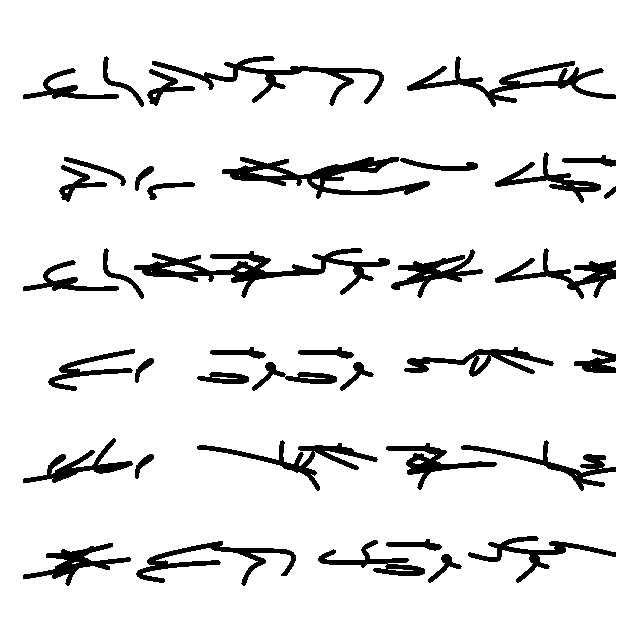
\includegraphics[width=3.5in]{tweaked.png}
	\vspace{-18pt}
	\caption{Different parameters to the \texttt{Handwriting} class}
	\label{tweaked}
\end{figure}
\vfill
\bibliographystyle{acm}
\bibliography{writeup}

\end{document}
